\documentclass[a4paper,11pt]{article}
\usepackage[T1]{fontenc}
\usepackage{hyperref}
\usepackage{titlesec}
\usepackage{graphicx}
\graphicspath{ {images/} }

%\titleformat{\subsection}
%[display]
%{\large\bfseries}
%{Exercise \thesubsection}{1pt}{}

% Star to kill indentation of following par.
%\titlespacing*{\subsection}
%{0pt}{5pt}{-15pt}


\titleformat{\section}
[runin]
{\LARGE\bfseries}
{Exercise \thesection: \rightmark}{1pt}{}

\titleformat{\subsection}
{\large\bfseries}
{Sub-exercise \thesubsection}{1pt}{}

% Star to kill indentation of following par.
\titlespacing*{\subsection}
{0pt}{5pt}{0pt}

\title{TI2206 Software Engineering \\ Bubble Shooter report: Assignment 1 \\ EEMCS/EWI}
\author{Gerlof Fokkema 4257286 \\
	Owen Huang 4317459 \\
	Adam Iqbal 4293568 \\
	Nando Kartoredjo 4271378 \\
	Skip Lentz 4334051 \\
}

\begin{document}
\maketitle
\thispagestyle{empty}

\newpage
\setcounter{page}{1}

%###################################### EXERCISE 1 ###################################### 
\section{The core \\}
In this section the exercises 1.1 up to 1.4 are elaborated with fully in depth explanations. \\

%~~~~~~~~~~~~ SUB-EXERCISE 1.1 ~~~~~~~~~~~~
\subsection{}
The two \textbf{main} classes that have already been implemented, described in terms of responsibility and collaborations are as follows:
\begin{enumerate}
  \item First, one of the most important classes is the \textit{Board} class. This class describes the entire playing-field. It can also place and remove bubbles, and it can return the clusters of bubbles of the same color. It collaborates with the \textit{BubbleShooterScreen} class and the \textit{Bubble} class.
  \item Secondly, the \textit{BubbleShooterScreen} class should also be considered one of the main classes. It is responsible for drawing all the game elements (bubbles, cannon and background) onto the screen, for the game logic and for applying the game's rules. Additionally it takes care of the user input and acts accordingly. It collaborates with the \textit{Board} class and the \textit{Cannon} class.
\end{enumerate}

%~~~~~~~~~~~~ SUB-EXERCISE 1.2 ~~~~~~~~~~~~
\subsection{}
The reason why the other classes are not considered main classes, is because of the fact that they carry far less responsibility. Those classes do not collaborate with that many classes in comparison to the main classes. For example, the \textit{Bubble} class does not "know" about any other classes, and its only responsibility is basically to exist.\\\\
\noindent
Looking at the current structure, some changes to the non-main classes are in order.

First up are the \textit{BackgroundMusic} and \textit{SoundEffect} classes. These two classes both take care of the audio of the application. While it is not necessarily bad to have these two seperate, the responsibility these two classes have are somewhat similar; one manages the background music and the other the various sound effects. As previously mentioned, this simply relates to the audio. So these classes can be easily merged together into one larger class: the \textit{SoundEngine}.

The next issue, that should be addressed, is loading assets into the game. At first this was just done in every single class where the asset was necessary itself. This caused everything to become rather cluttered, so it would make sense to do all the asset loading in another place. This resulted into introducing a new class: the \textit{Assets} class. All the assets would then be loaded from the start of the application in the \textit{Launch} class.
 \newpage
%~~~~~~~~~~~~ SUB-EXERCISE 1.3 ~~~~~~~~~~~~
\subsection{}
\begin{figure}[h]
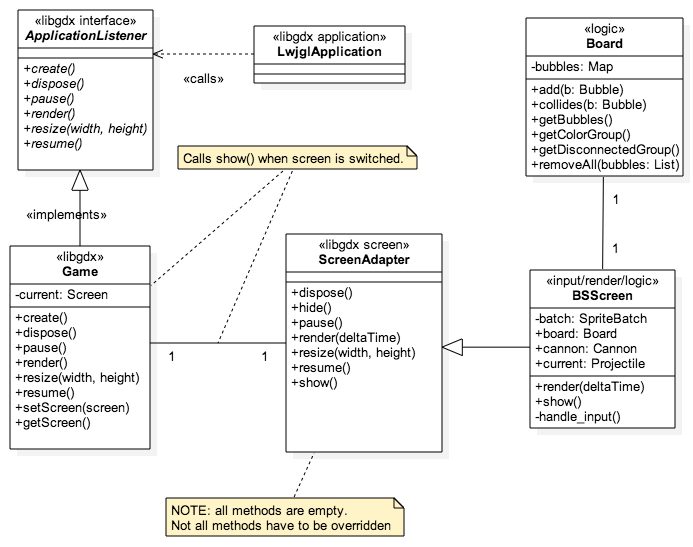
\includegraphics[width=\textwidth]{old_class_diagram}
\caption{The class diagram after the first sprint}
\end{figure}
\newpage
%~~~~~~~~~~~~ SUB-EXERCISE 1.4 ~~~~~~~~~~~~
\subsection{}
\begin{figure}[h]
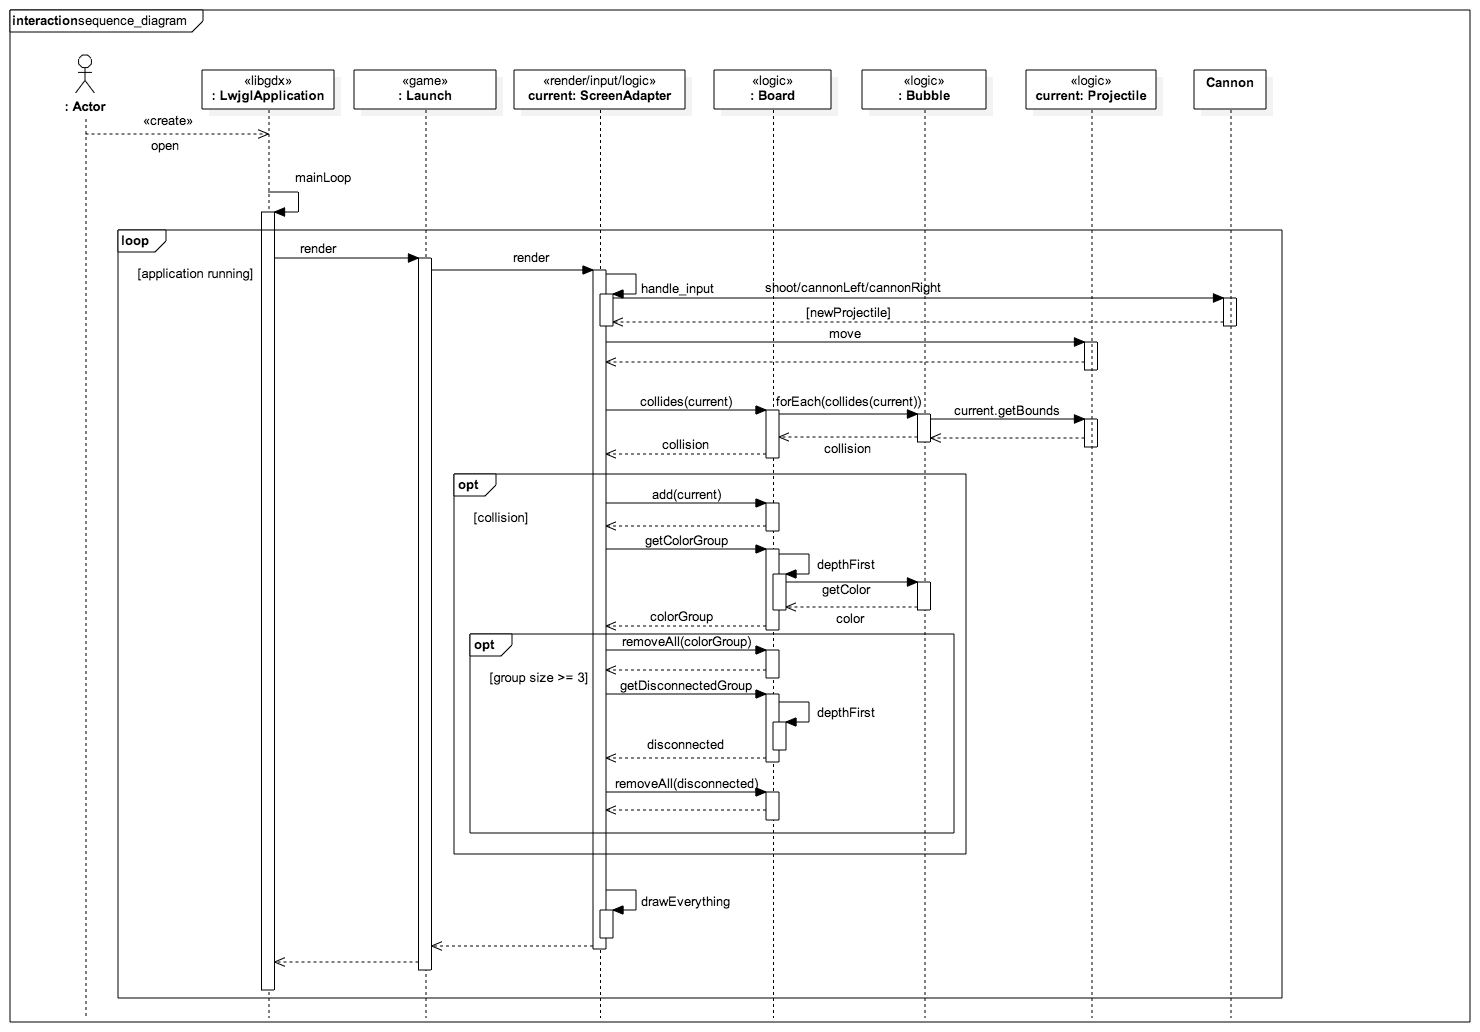
\includegraphics[width=\textwidth]{old_sequence_diagram}
\caption{The sequence diagram after the first sprint}
\end{figure}
%###################################### EXERCISE 2 ###################################### 
\section{Theory in practice \\}

In this section the exercises 2.1 up to 2.3 are elaborated with fully in depth explanations. \\

%~~~~~~~~~~~~ SUB-EXERCISE 2.1 ~~~~~~~~~~~~
\subsection{}
\begin{enumerate}
  \item \textbf{Aggregation} is a special form of \textbf{association}. This is best described as a `has-a' relationship between a parent and the child, meaining that the child does not necessarily need the parent in order to simply exist.
  \item \textbf{Composition} is a special form of \textbf{aggregation}. This differs from aggregation, in the following: the relationship between the parent and child will not hold when the parent does no longer exist. In other words, the child may not exist without its parent.
\end{enumerate}
Inside the project, there are two cases of \textbf{composition} to be found.
\par Firstly, the \textit{Bubble} class has such a relationship with the \textit{Board} class. The \textit{Board} contains lots of bubbles, so when the board stops existing so do all the bubbles.
\par Secondly, the various classes that adapt the \textit{ScreenAdapter} class, such as the \textit{MainMenuScreen}, have a similar relationship with the \textit{Button} class. When the main menu vanishes, the buttons follow. \\\\
Furthermore, several cases of aggregation also occur. However these relationships currently exist, they are not favorable and should be changed later on (because it does not hold a `logical connection' with the corresponding classes). These relationships can be found inside the \textit{BubbleShooterScreen} class. The \textit{BubbleShooterScreen} currently holds three \textit{aggregation} relationships with the \textit{Cannon}, \textit{Board} and \textit{Projectile} classes. This is due to the fact that the \textit{BubbleShooterScreen} contains these elements, however they do not necessarily need the \textit{BubbleShooterScreen} in order to exist.


%~~~~~~~~~~~~ SUB-EXERCISE 2.2 ~~~~~~~~~~~~
\subsection{}
\begin{figure}[h]
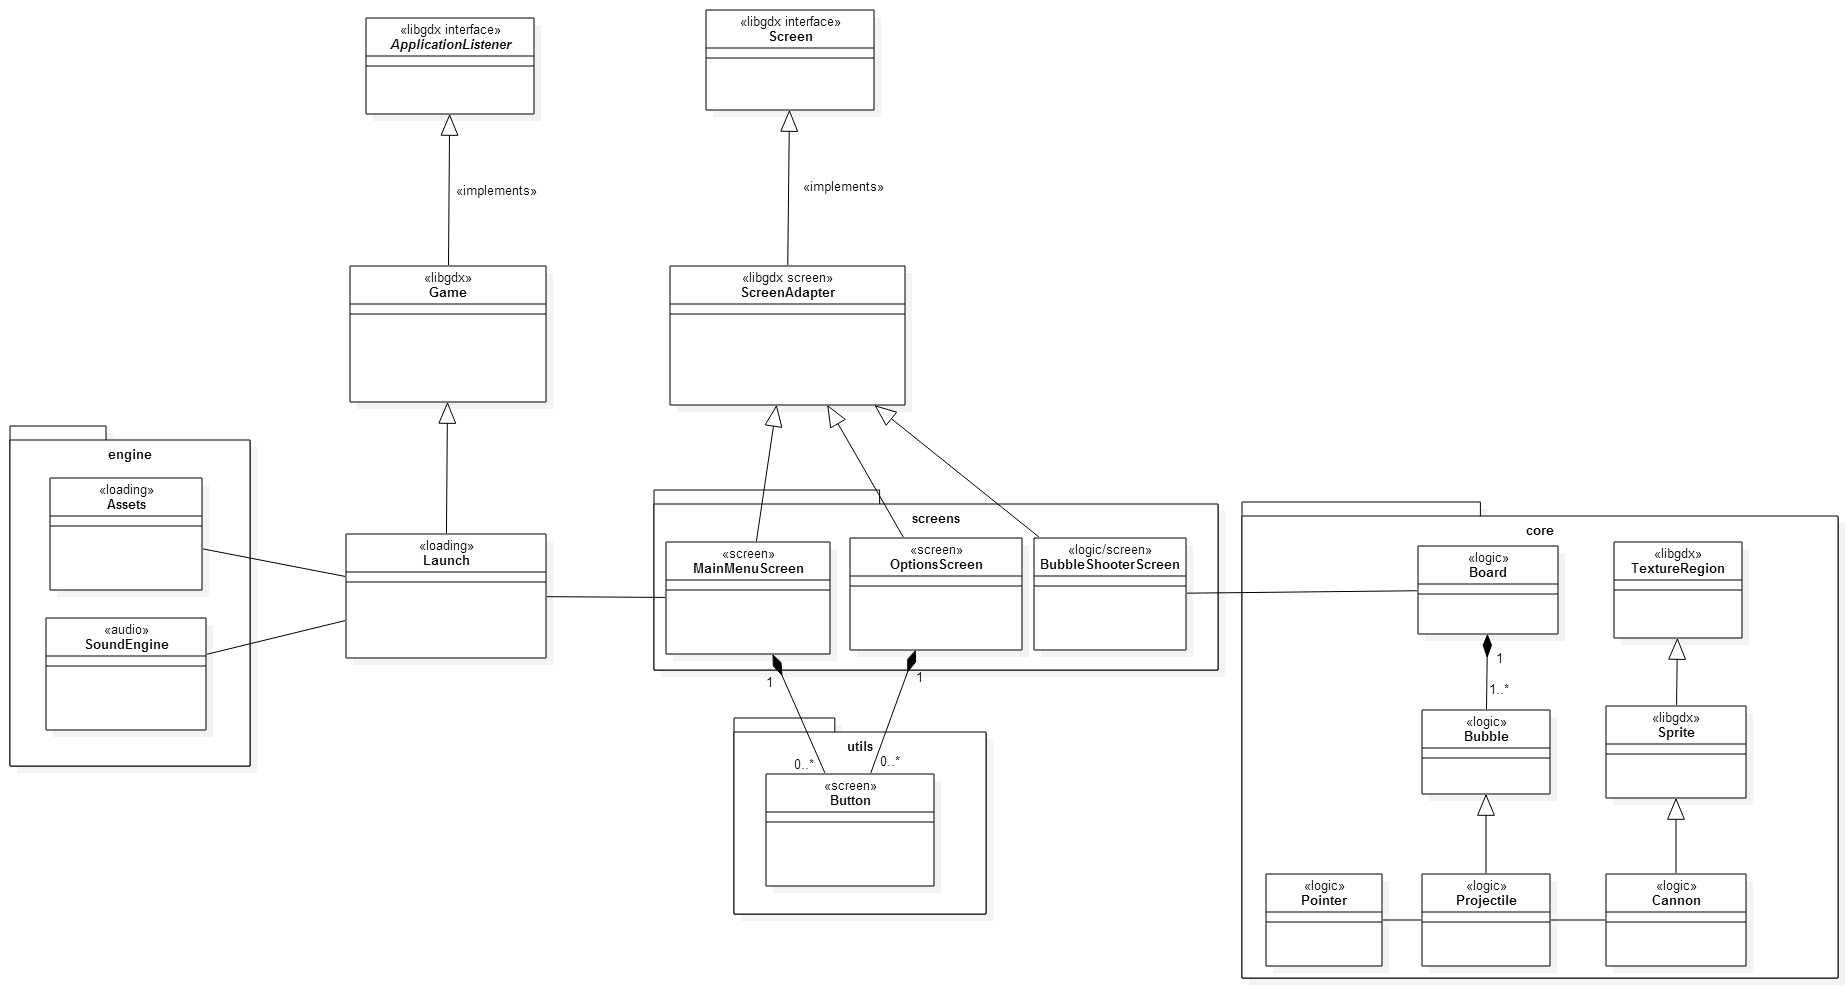
\includegraphics[width=\textwidth]{class_hierarchy}
\caption{The class hierarchy at the current state}
\end{figure}
The following class hierarchy was made without a lot of careful thinking beforehand. So it was mostly done on a whim. The various kinds of relationships are also marked in the diagram with different symbols. The black diamond is a composition relationship, the arrow is a generalization (which indicates subclassing). Furthermore the regular line is a association. The \textit{Board} and \textit{Bubble} relationship was also explained in \textbf{Sub-Exercise 2.1}, this also goes for the \textit{Screen} classes (including the \textit{Button}).

%~~~~~~~~~~~~ SUB-EXERCISE 2.3 ~~~~~~~~~~~~
\subsection{}
There are cases of if-statements to be found in the project. Most if-statements from the \textit{BubbleShooterScreen} have been refactored. A new structure for handling user input has been introduced to reduce the amount of if-statements: these include the \textit{AbstractProcessor} and the \textit{SinglePlayerProcessor} classes. Instead of checking every time whether a given key has been pressed, all the keybindings are put into a Map. Only a single lookup into the map has to be done, in order to check if there has to be some kind of response to the user input.
\par Other cases where if-statements were used, should remain. This is because there is no valid reason to replace them, because there is no profit to gain from doing so. Additionally these if-statements are not if-statements, that are `out of place'. They provide structure to the code and cannot be replaced by f.e: a polymorphic structure.

%###################################### EXERCISE 3 ###################################### 
\section{Play with your friends}
%#nofrends#foreveralone

%~~~~~~~~~~~~ SUB-EXERCISE 3.1 ~~~~~~~~~~~~
\subsection{}
The implementation can be found in the attached files.
%~~~~~~~~~~~~ SUB-EXERCISE 3.2 ~~~~~~~~~~~~
\subsection{}
The documents derived during this phase can also be found in the same place as previously mentioned. This is a snapshot moment.\\
\begin{figure}[h]
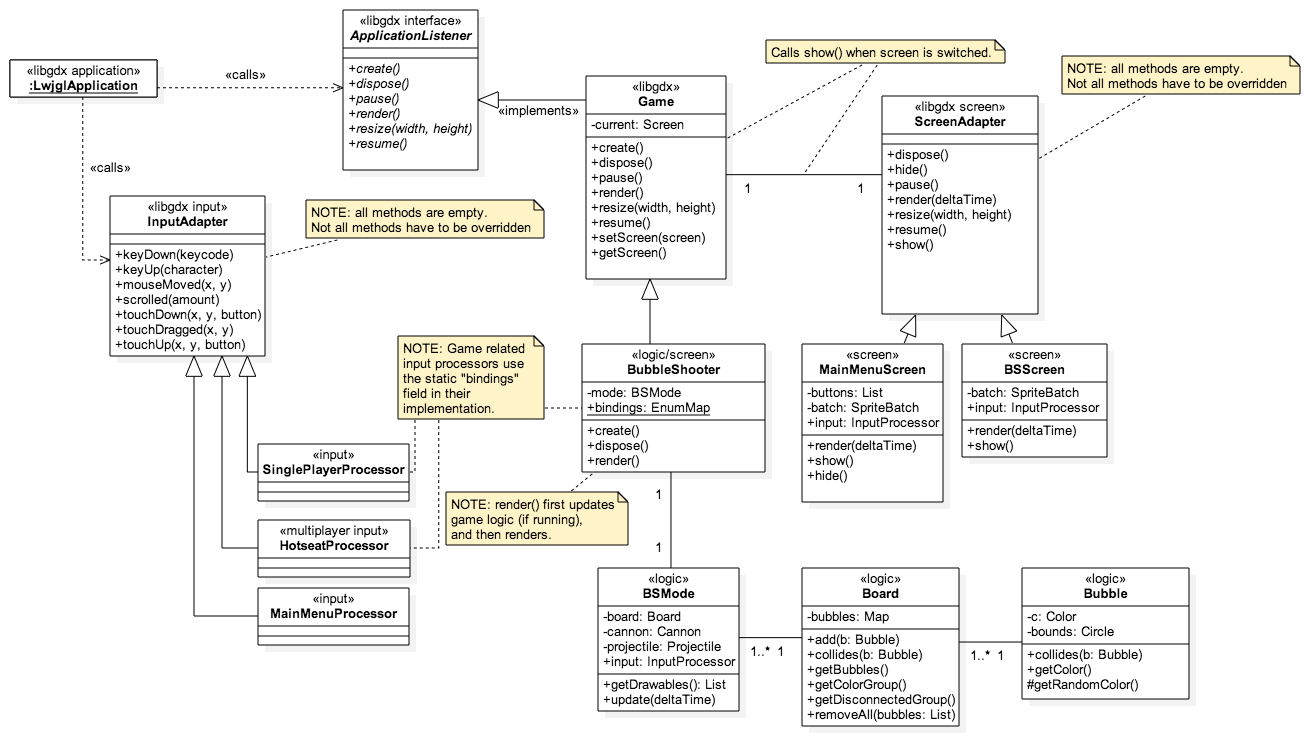
\includegraphics[width=\textwidth]{new_class_diagram}
\caption{A snapshot moment from the new class diagram}
\end{figure}
\begin{figure}[h]
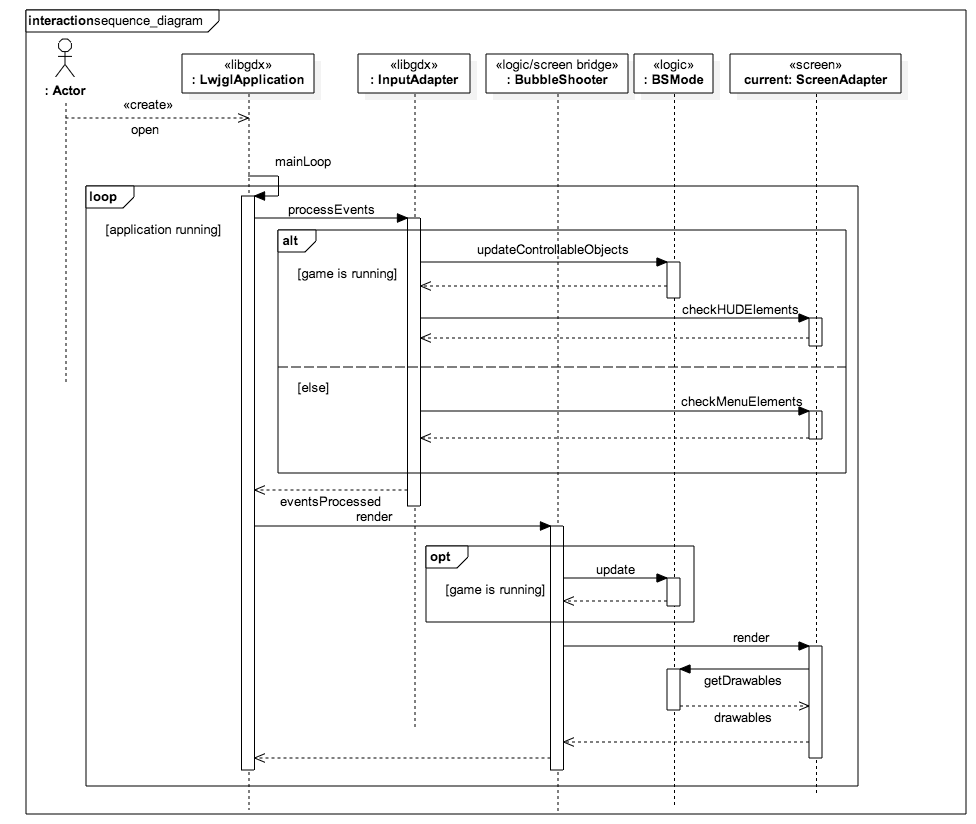
\includegraphics[width=\textwidth]{new_sequence_diagram}
\caption{A snapshot moment from the new sequence diagram}
\end{figure}

\end{document}